\documentclass{beamer}
\usetheme{Warsaw}
\usepackage{graphicx}
\usepackage[german]{babel}
\usepackage[T1]{fontenc}
\usepackage[utf8]{inputenc}

\title{Umgang mit Sozialen Netzwerken}
\author{Chaos Computer Club Dresden}
\date{\today}

\begin{document}
\maketitle
\frame{\tableofcontents}

\section{Meta}

\begin{frame}
  \frametitle{Wer sind wir?}
  \begin{itemize}
    \item<1-> Chaos Computer Club Dresden
    \item<2-> Datenspuren
    \item<3-> Podcasts
    \item<4-> Chaos macht Schule
  \end{itemize}
\end{frame}

\begin{frame}
  \frametitle{Unser Anliegen}
  \begin{itemize}
    \item<1-> Kinder auf das Internet vorbereiten ...
    \item<2-> ... nicht das Internet auf Kinder
    \item<3-> Medienkompetenz
    \item<4-> Kreativer Umgang mit Technik
  \end{itemize}
\end{frame}

\section{Internet}

\begin{frame}
  \frametitle{Grundlagen des Internets}
  \begin{itemize}
    \item<1-> Dezentralität
    \item<2-> Jeder ist Sender und Empfänger
    \item<3-> Verlinkung
    \item<4-> Pseudonymität
  \end{itemize}
\end{frame}

\begin{frame}
  \frametitle{Probleme des Internets}
  \begin{itemize}
    \item<1-> Ungeschützte Datenübertragung
    \item<2-> Keine Authentifizierung
    \item<3-> "Das Internet vergisst nicht"
  \end{itemize}
\end{frame}

\begin{frame}
  \frametitle{Praxis}
  Kindernet
\end{frame}

\begin{frame}
  \frametitle{Historie des Internets}
  \begin{itemize}
    \item<1-> Web 1.0
    \item<2-> Zulauf von Firmen und Allgemeinheit
    \item<3-> Web 2.0
  \end{itemize}
\end{frame}

\section{Soziale Netzwerke}

\begin{frame}
  \frametitle{Soziale Netzwerke (1)}
  \begin{figure}
    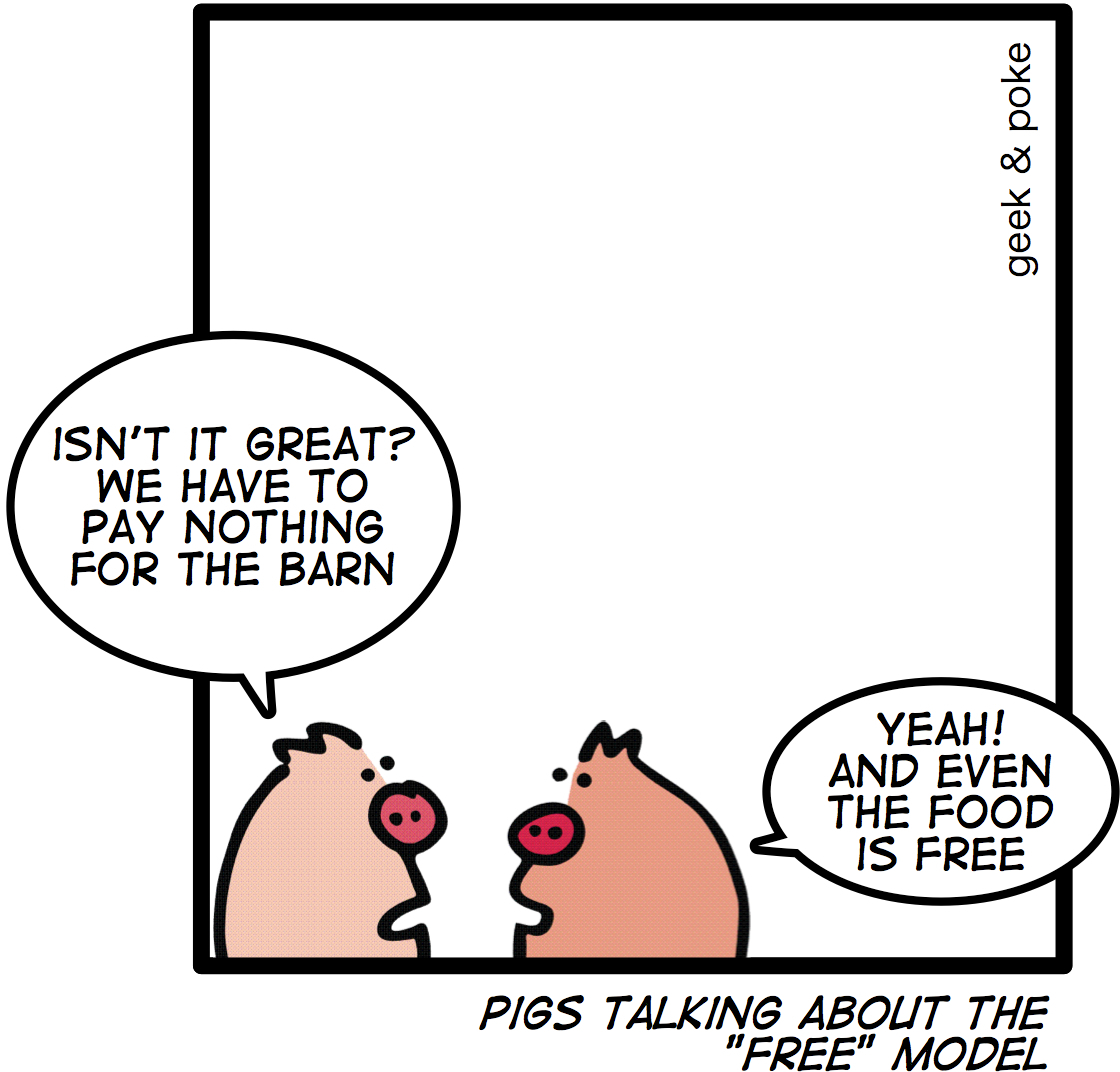
\includegraphics{img/business_pigs.jpg}
    \caption{CC-BY-SA http://geekandpoke.typepad.com/geekandpoke/2010/12/the-free-model.html}
  \end{figure}
\end{frame}

\begin{frame}
  \frametitle{Soziale Netzwerke (2)}
  \begin{itemize}
    \item<1-> Zentralität
    \item<2-> Identität
    \item<3-> Was bedeutet "Befreundet sein"?
    \item<4-> gerichtete/ungerichtete Graphen
  \end{itemize}
\end{frame}

\begin{frame}
  \frametitle{Praxis}
  Kinderbook
\end{frame}

\section{Freiheit}

\begin{frame}
  \frametitle{Back to the Basics}
  \begin{itemize}
    \item<1-> Alle Sender gleichberechtigt
    \item<2-> Dezentrale Dienste
      \begin{itemize}
        \item<3-> Email
        \item<4-> Jabber/XMPP
        \item<5-> Diaspora, Buddycloud
      \end{itemize}
  \end{itemize}
\end{frame}

\begin{frame}
  \frametitle{Freie Lizenzen (1)}
  \begin{itemize}
    \item<1-> Jeder ist Produzent und Konsument
    \item<2-> Urheberrecht schränkt Verwendung ein
    \item<3-> Freie Lizenzen ermöglichen Verbreitung
    \item<4-> Sharing is caring
  \end{itemize}
\end{frame}

\begin{frame}
  \frametitle{Freie Medien}
  \begin{itemize}
    \item<1-> Freie Lehrmaterialien
    \item<2-> Freie Musik
      \begin{itemize}
        \item Jamendo
        \item Free Music Archive
        \item Pentamusic
      \end{itemize}
    \item<3-> OpenStreetMap
  \end{itemize}
\end{frame}

\begin{frame}
  \frametitle{Freie Software}
  \begin{itemize}
    \item Windows -> Linux
    \item Microsoft Office -> Libre Office/Open Office
    \item Internet Explorer -> Firefox
    \item Outlook -> Thunderbird
    \item Photoshop -> Gimp
    \item Illustrator -> Inkscape
    \item Windows Mediaplayer -> VLC Media Player
  \end{itemize}
\end{frame}

\section{Fazit}

\begin{frame}
  \frametitle{Fazit}
  \begin{itemize}
    \item So what?
  \end{itemize}
\end{frame}

\end{document}
